%% Creator: Inkscape inkscape 0.92.4, www.inkscape.org
%% PDF/EPS/PS + LaTeX output extension by Johan Engelen, 2010
%% Accompanies image file 'model.pdf' (pdf, eps, ps)
%%
%% To include the image in your LaTeX document, write
%%   \input{<filename>.pdf_tex}
%%  instead of
%%   \includegraphics{<filename>.pdf}
%% To scale the image, write
%%   \def\svgwidth{<desired width>}
%%   \input{<filename>.pdf_tex}
%%  instead of
%%   \includegraphics[width=<desired width>]{<filename>.pdf}
%%
%% Images with a different path to the parent latex file can
%% be accessed with the `import' package (which may need to be
%% installed) using
%%   \usepackage{import}
%% in the preamble, and then including the image with
%%   \import{<path to file>}{<filename>.pdf_tex}
%% Alternatively, one can specify
%%   \graphicspath{{<path to file>/}}
%% 
%% For more information, please see info/svg-inkscape on CTAN:
%%   http://tug.ctan.org/tex-archive/info/svg-inkscape
%%
\begingroup%
  \makeatletter%
  \providecommand\color[2][]{%
    \errmessage{(Inkscape) Color is used for the text in Inkscape, but the package 'color.sty' is not loaded}%
    \renewcommand\color[2][]{}%
  }%
  \providecommand\transparent[1]{%
    \errmessage{(Inkscape) Transparency is used (non-zero) for the text in Inkscape, but the package 'transparent.sty' is not loaded}%
    \renewcommand\transparent[1]{}%
  }%
  \providecommand\rotatebox[2]{#2}%
  \newcommand*\fsize{\dimexpr\f@size pt\relax}%
  \newcommand*\lineheight[1]{\fontsize{\fsize}{#1\fsize}\selectfont}%
  \ifx\svgwidth\undefined%
    \setlength{\unitlength}{443.15460926bp}%
    \ifx\svgscale\undefined%
      \relax%
    \else%
      \setlength{\unitlength}{\unitlength * \real{\svgscale}}%
    \fi%
  \else%
    \setlength{\unitlength}{\svgwidth}%
  \fi%
  \global\let\svgwidth\undefined%
  \global\let\svgscale\undefined%
  \makeatother%
  \begin{picture}(1,0.56587843)%
    \lineheight{1}%
    \setlength\tabcolsep{0pt}%
    \put(0,0){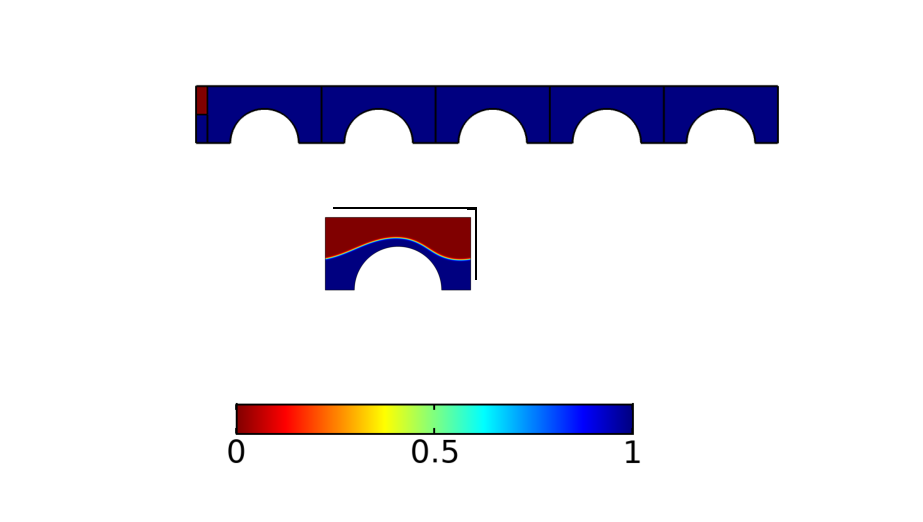
\includegraphics[width=\unitlength,page=1]{model.pdf}}%
    \put(0.26660576,0.47767245){\color[rgb]{0,0,0}\makebox(0,0)[lt]{\lineheight{1.25}\smash{\begin{tabular}[t]{l}UC1\end{tabular}}}}%
    \put(0.3869981,0.47767245){\color[rgb]{0,0,0}\makebox(0,0)[lt]{\lineheight{1.25}\smash{\begin{tabular}[t]{l}UC2\end{tabular}}}}%
    \put(0.51077273,0.47767245){\color[rgb]{0,0,0}\makebox(0,0)[lt]{\lineheight{1.25}\smash{\begin{tabular}[t]{l}UC3\end{tabular}}}}%
    \put(0.63597003,0.47767245){\color[rgb]{0,0,0}\makebox(0,0)[lt]{\lineheight{1.25}\smash{\begin{tabular}[t]{l}UC4\end{tabular}}}}%
    \put(0.75774814,0.47767245){\color[rgb]{0,0,0}\makebox(0,0)[lt]{\lineheight{1.25}\smash{\begin{tabular}[t]{l}UC5\end{tabular}}}}%
    \put(0,0){\includegraphics[width=\unitlength,page=2]{model.pdf}}%
    \put(0.09645976,0.44349829){\color[rgb]{0,0,0}\makebox(0,0)[lt]{\lineheight{1.25}\smash{\begin{tabular}[t]{l}Inlet $o$\end{tabular}}}}%
    \put(0.09298877,0.4102802){\color[rgb]{0,0,0}\makebox(0,0)[lt]{\lineheight{1.25}\smash{\begin{tabular}[t]{l}Inlet $w$\end{tabular}}}}%
    \put(0,0){\includegraphics[width=\unitlength,page=3]{model.pdf}}%
    \put(0.8619084,0.3923161){\color[rgb]{0,0,0}\makebox(0,0)[lt]{\lineheight{1.25}\smash{\begin{tabular}[t]{l}Outlet\end{tabular}}}}%
    \put(0,0){\includegraphics[width=\unitlength,page=4]{model.pdf}}%
    \put(0.30230707,0.50596373){\color[rgb]{0,0,0}\makebox(0,0)[lt]{\lineheight{1.25}\smash{\begin{tabular}[t]{l}Symmetry\end{tabular}}}}%
    \put(0,0){\includegraphics[width=\unitlength,page=5]{model.pdf}}%
    \put(0.66206543,0.34010743){\color[rgb]{0,0,0}\makebox(0,0)[lt]{\lineheight{1.25}\smash{\begin{tabular}[t]{l}Symmetry\end{tabular}}}}%
    \put(0.22252169,0.26704458){\color[rgb]{0,0,0}\makebox(0,0)[lt]{\lineheight{1.25}\smash{\begin{tabular}[t]{l}$w$-phase\end{tabular}}}}%
    \put(0.23029302,0.30197361){\color[rgb]{0,0,0}\makebox(0,0)[lt]{\lineheight{1.25}\smash{\begin{tabular}[t]{l}$o$-phase\end{tabular}}}}%
    \put(0,0){\includegraphics[width=\unitlength,page=6]{model.pdf}}%
    \put(0.48064022,0.36146904){\color[rgb]{0,0,0}\makebox(0,0)[lt]{\lineheight{1.25}\smash{\begin{tabular}[t]{l}$h$\end{tabular}}}}%
    \put(0,0){\includegraphics[width=\unitlength,page=7]{model.pdf}}%
    \put(0.41423405,0.23059471){\color[rgb]{0,0,0}\makebox(0,0)[lt]{\lineheight{1.25}\smash{\begin{tabular}[t]{l}$A_{ws}$\end{tabular}}}}%
    \put(0,0){\includegraphics[width=\unitlength,page=8]{model.pdf}}%
    \put(0.52145744,0.22080229){\color[rgb]{0,0,0}\makebox(0,0)[lt]{\lineheight{1.25}\smash{\begin{tabular}[t]{l}$A_{wo}$\end{tabular}}}}%
    \put(0,0){\includegraphics[width=\unitlength,page=9]{model.pdf}}%
    \put(0.52647077,0.29650035){\color[rgb]{0,0,0}\rotatebox{-179.3987}{\makebox(0,0)[lt]{\lineheight{1.25}\smash{\begin{tabular}[t]{l}$l$\\\end{tabular}}}}}%
    \put(0.37233056,0.14264612){\color[rgb]{0,0,0}\makebox(0,0)[lt]{\lineheight{1.25}\smash{\begin{tabular}[t]{l}Volume fraction\end{tabular}}}}%
  \end{picture}%
\endgroup%
